\section{Restoring Force Surface}
\label{sec:rfs_description}

The restoring force surface (RFS) method, introduced by \cite{masri1979a} and
covered in details in \autocite{worden1990a}, have previously been used
as a parameter estimation technique, but is only used as a visual tool for
characterization the functional form of the nonlinearity in this report.

If RFS is used for parameter estimation, an estimation of the inertia for the
system is needed. This either requires an FE model or, for more than a few DOFs,
an complicated algebraic model. If an FE model is used, a low level test campaign
could be used to calibrate the model until it fits the experimental
eigenfrequencies.

(\autocite{masri2004a} demonstrates a generalisation of the RFS which estimates
parameters exclusively from time signals, but the method is only applicable to
systems with a few DOFs since the method still consist of direct fitting of
Newton's second law.)


The starting point is Newton's second law of dynamics written for a specific DOF
located next to a nonlinear structural component

\begin{equation}
  \label{eq:rfs_newton}
  \sum_{k=1}^{n} m_{i,k} \ddot x_k + g_i(\bm x, \dot{ \bm x}) = f_i
\end{equation}

where $i$ is the DOF of interest, $n$ the number of DOFs in the system, $m_{ik}$
the mass matrix elements, $\bm x$, $\dot{\bm x}$ and $\ddot{ \bm x}$ the
displacement, velocity and acceleration vectors, respectively, $\bm g$ the
restoring force vector encompassing elastic and dissipative effects, and $\bm f$
the external force vector.

The difference between the traditional usage of RFS, to this approach is to
discard any restoring force or inertia terms that are not directly connected to
the nonlinear component. (\textit{The discarded terms are generally unknown
  terms which are practically impossible to measure in an experiment, such as
  the coupling inertia coefficients and the rotational DOF.})

If $j$ denote another measured DOF located across the nonlinear connection, see
figure \ref{fig:rfs_schematic}, a new formulation of \eqref{eq:rfs_newton},
which accounts for the difference in displacement and velocity between the
selected DOFs, is approximated with

\begin{equation}
  \label{eq:rfs_newton2}
  m_{i,j} \ddot x_i +  g_i (x_i - x_j , \dot x_i - \dot x_j) \approx f_i
\end{equation}

\begin{figure}[ht!]
  \centering
  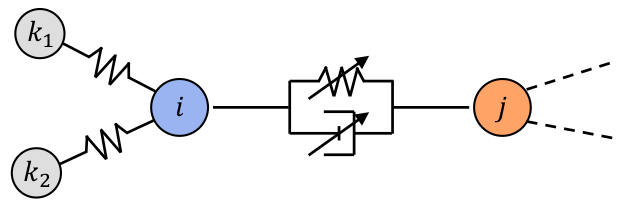
\includegraphics[width=0.5\textwidth]{rfs/rfs_schematic.png}
  \caption{Nonlinear connection between node $i$ and $j$. The linear connections
    to $k_{1,2}$ are discarded.}
  \label{fig:rfs_schematic}
\end{figure}

It is further assumed that no external force is applied directly at DOF $i$
(eg. the external force is applied at a different location on the structure), an
rearrangement leads to
\begin{equation}
  \label{eq:rfs}
  g_i (x_i - x_j , \dot x_i - \dot x_j) \approx -m_{i,j} \ddot x_i
\end{equation}

Thus by dropping the constant mass, the nonlinearities can be visualized as the
negative acceleration at one side of the connection, as a function of the
relative displacement and velocity across this connection. From this an adequate
mathematical model can be found.

The shape of $g$ is visualized by plotting the triplet
$(x_{i,k} - x_{j,k}, \dot x_{i,k} - \dot x_{j,k}, \ddot x_{i,k})$, where $k$
is the  $k$'th sampled instant.
The form of elastic (dissipative) nonlinearities in the connection is visualized
by making a slice along the axis of the zero velocity (displacement) of the
restoring force surface plot.
Either prior knowledge about the physics or a least square fit can be
used to find the functional that best represent the nonlinearity.

%The velocity and displacement are found by numerical integration, see section
%\ref{chap:signals}.


The major limitations of the RFS method is
\begin{itemize}
\item Requires the nonlinear dynamics to be excited
\item Shows the total restoring force:
  \begin{itemize}
  \item with multiple nonlinearities it is not possible to distinguish them
    uniquely.
  \item If the nonlinear force is of the same magnitude as the linear force, it
    might be necessary to remove a linear trend from the RFS to visualise the
    nonlinear force.
  \end{itemize}
\item Works best swept-sine excitation.
\item Damping characterisation is difficult due to the low numerical magnitude.
\end{itemize}


\subsection{Example}
\label{sec:rfs_example}

Using a sine sweep excitation on the coupled duffing system and the RFS
methodology,
\begin{equation}
  \label{eq:rfs_tol}
  g_i (x_i - x_j , \underbrace{\dot x_i - \dot x_j}_\text{<tol}) \approx - \ddot x_i
\end{equation}
where \textit{tol} determines the slice thickness, the restoring force is
visualised in figs \ref{fig:rfs_full} and \ref{fig:rfs_stiff} for $x_0$ and
$x_1$. A hardening stiffness is seen, without any offset, which correspond to a
uneven nonlinear polynomial stiffness. In this case a third order polynomial for
both DOFs.

\begin{figure}[!ht]
  \centering
  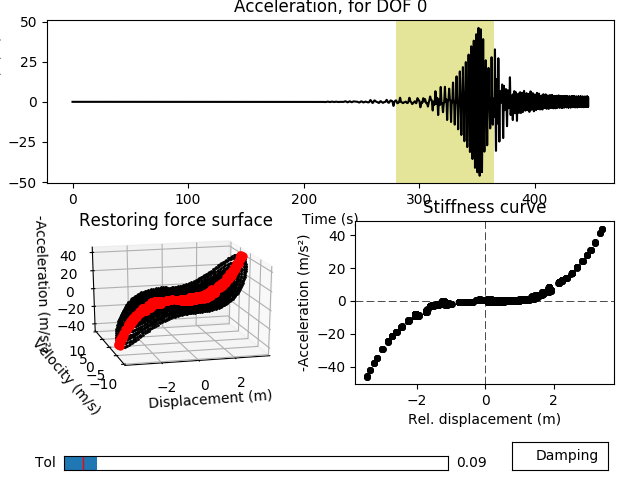
\includegraphics[width=0.8\textwidth]{rfs/sweepvrms3dof0_rfs.png}
  \caption{Interface for selecting the part of the signal used for
    visualising the restoring force of the coupled duffing system. Here shown
    for $x_1$.
    \textbf{upper}: The relevant part of the signal is selected by dragging or
    resizing the yellow rectangle;
    \textbf{left}: Restoring force surface for the selected part of the signal.
    The red line shows the slice;
    \textbf{right}: The visualised stiffness. The slice thickness can be changed
    by dragging the tolerance slider. Damping is visualised by clicking on
    damping.
  }
  \label{fig:rfs_full}
\end{figure}


\begin{figure}[!ht]
  \centering
  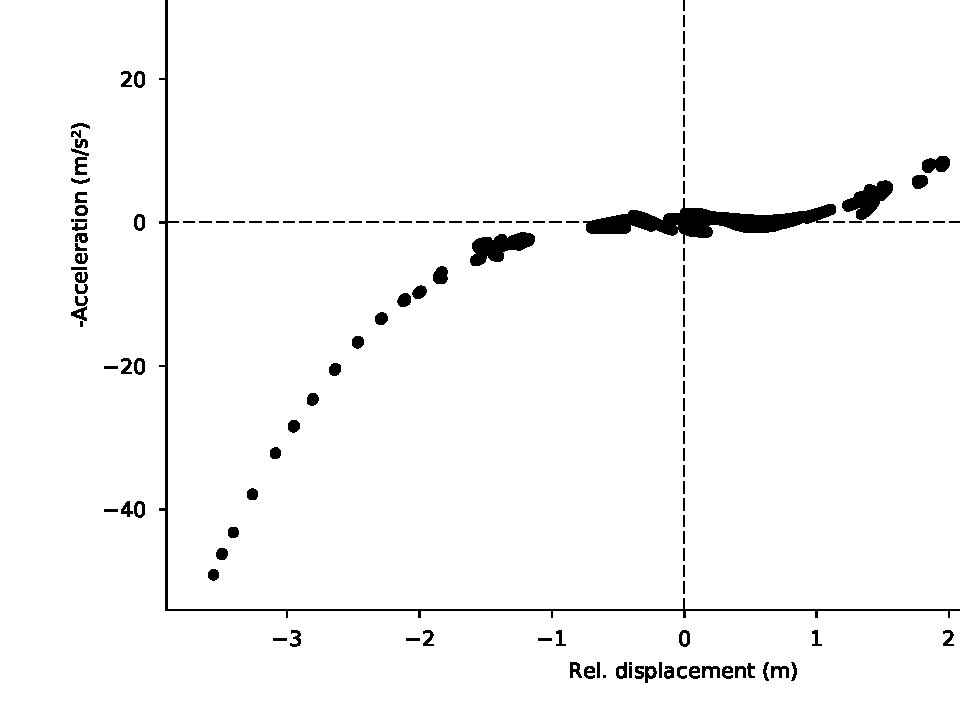
\includegraphics[width=0.6\linewidth, height=6cm]{rfs/sweepvrms3dof1_stiff}
  \caption{The visualised stiffness for $x_2$ from the coupled duffing system.
    The figure is extracted from the interface shown in fig. \ref{fig:rfs_full};
    just for $x_2$ instead}
  \label{fig:rfs_stiff}
\end{figure}

\subsection{Summary}
\label{sec:rfs_summary}

The RFS provides a direct visualization of the nonlinear stiffness and, to
lesser extend, damping curve using a SDOF simplification of the EOMs. The steps
are:
\begin{itemize}
\item Instrument the nonlinear connection with two accelerometers and use swept
  sine excitation.
\item Integrate and filter to obtain displacement and velocity.
\item Calculate the 3D acceleration surface over a single connection.
\item Make surface slides to obtain stiffness and damping curve.
\end{itemize}

The advantages of RFS as presented here, is that it relies exclusively on measured
time series and have a visual understanding. It is not commonly used for
parameter estimation for MDOF systems, due to the need for direct fitting of
Newton's second law.

The RFS method have been used for estimation of MDOF
systems\autocite{dossogne2015a,noel2014_phd}. But in the former, the complete
mass, damping and stiffness matrices are known from a detailed FE model and in
the latter, the complete equation of motion for the MDOF system are
derived a priory to the estimation.

The success of parameter estimation step is conditional upon an accurate
characterization of all observed nonlinearities.
RFS is also called Accelerated Surface Method (ASM) at times in literature.


%%% Local Variables:
%%% mode: latex
%%% TeX-master: "../../report"
%%% End:
